\section{Durchführung}
\label{sec:Aufbau und Durchführung}
Zu Beginn werden alle Figuren mehrmals vermessen und gewogen, anschließend wird der Mittelwert bestimmt.
\subsection{Bestimmung der Winkelrichtgröße $D$ und des Eigenträgheitsmomentes $I_{\mathrm{D}}$ der Drillachse}
Ein als masselos angenommener Stab wird in folgende Apparatur eingespannt:
  \begin{figure}[h]
      \centering
      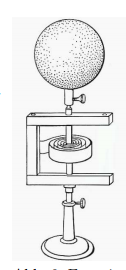
\includegraphics[width=0.3\textwidth]{Apparatur.PNG}
      \caption{Apparatur zur Vermessung der Trägheitsmomente.\cite{skript}}
      \label{abb:apparatur}
  \end{figure}\\
\subsubsection{Statistische Methode}
Der Stab wird mit einer Federwage um verschiedene Winkel $\varphi$ senkrecht zum Bahnradius ausgelenkt.
Notiert werden der Abstand $r$ zur Drehachse, die gemessene Kraft $F$ und der Winkel $\varphi$.
Die Messung wird für zehn verschiedene Auslenkwinkel durchgeführt.

\subsubsection{Dynamische Methode}
Zur bestimmung von $I_{\mathrm{D}}$ werden zwei ähnliche Gewichte auf den Stab gespannt. Der Stab wird dann ausgelenkt und
die Schwingungsdauer für fünf Schwingungsperioden wird mit einer Stoppuhr erfasst.
Dies geschieht für 10 verschiedene Abstände der Gewichte zur Drechachse.

\subsection{Trägheitsmoment von geometrischen Figuren}
Das Trägheitsmoment für die weiße Kugel und den schwarzen Zylinder werden nach dem dynamischen Verfahren bestimmt. Dazu werden die Figuren jeweils auf die Drillachse gespannt,
dann wird die Figur ausgelenkt und die Schwingungsdauer für fünf Schwingungsperioden gestoppt. Diese Messung wird zehn mal durchgeführt.

\subsection{Trägheitsmoment einer Puppe}
Für die Messung wird die Puppe in zwei verschiedene Positionen gebracht und die Schwingungsdauer für fünf Perioden aufgenommen.
Jeweils zehn mal wird die Schwingungsdauer vermessen für beide Positionen. Die Puppe wird zum einen mit anliegenden Armen und runtergeklappten Füßen auf die Drillachse gespannt
und zum anderen mit seitlich ausgestreckten Armen, sodass sie ein Kreuz beschreibt, eingespannt.
